
\section{Methodology}
\label{sec:method}

\subsection{Simulation Environment and Network}
\label{sec:method:net}

Experiments use SUMO~1.27.1 with a one-second step and vehicle teleporting
disabled \citep{lopez2018sumo}, so a vehicle that cannot enter the network waits
and remains in the accounting rather than being removed from it. Emissions use
the HBEFA3 \texttt{PC\_G\_EU4} model \citep{krajzewicz2015emissions} over a
homogeneous fleet.

The network (Fig.~\ref{fig:network}a) is a single origin--destination corridor
served by three parallel routes between a diverge and a merge. The central
arterial C is the shortest (3000\,m, two lanes, four signalised junctions); the
north street N is longer and slower (3242\,m, one or two lanes, four signalised
junctions); the south bypass S is longest but uninterrupted (3963\,m, one lane,
unsignalised). Because every junction permits straight-through movements only,
the set of loopless paths from the origin portal to the destination portal is
exactly $\{\mathrm{C},\mathrm{N},\mathrm{S}\}$. The candidate catalogue is
therefore complete rather than a $k$-shortest-path approximation, which removes
one degree of freedom from the comparison: no policy can be advantaged by a
better path-generation heuristic.

The three routes differ on the dimensions that make policy choice non-trivial:
C has the highest capacity but is signal-interrupted and is the target of every
distance-minimising assignment; N adds capacity only when it has two lanes; S
has fixed capacity and no signal variance, so it is the reliable option. Corridor
capacities were measured rather than assumed, by saturation-flow calibration runs
reported with the scenario. Cross-street background demand is held fixed so that
it does not confound the factorial. The three corridors share only the access and
egress links, so a route-overlap index carries no information and is not used.

Each run simulates a warm-up followed by a measurement window; the measured
cohort is every vehicle, guided or not, corridor or cross-street, with intended
departure in the window. Using the system-wide cohort rather than the guided
cohort is deliberate: a policy that improves guided vehicles by displacing
congestion onto others should not be credited for it.

\begin{figure}[htbp]
\centering
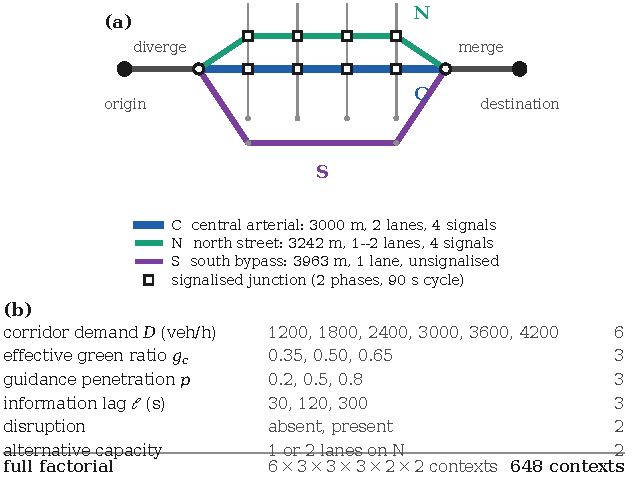
\includegraphics[width=\linewidth]{figures/fig1_network_design.pdf}
\caption{(a) The network. A single origin--destination corridor is served by
three parallel routes between the diverge and the merge: the short signalised
arterial C, the longer signalised street N, and the long unsignalised bypass S.
Cross streets carry fixed background demand. (b) The experimental factors and
their levels. The full factorial gives 648 contexts, each simulated under four
policies with five paired seeds.}
\label{fig:network}
\end{figure}

\subsection{Routing Policies}
\label{sec:method:pol}

All four policies choose one element of the three-path catalogue for one vehicle
at its moment of insertion. Three of them read traffic state, and they read it
from one shared observation buffer, so no policy has an information advantage
over another. The buffer stores the instantaneous travel time of every corridor
edge at a 30\,s sampling interval. A policy acting at time $t$ may read only
samples with timestamp at most $t-\ell$, where $\ell$ is the context's
information lag, and only the most recent 120\,s of those. Before any admissible
sample exists it falls back to free-flow times. No policy sees the future, and
none sees any realised outcome of the run it belongs to. Table~\ref{tab:policies}
states each policy; the parameters were frozen before any evaluation run and are
varied only in the sensitivity experiment of Section~\ref{sec:design:sens}.

\begin{table}[htbp]
\centering\small
\caption{The four routing policies. $L(p)$ is path length; $\hat\mu_p$ and
$\hat\sigma_p$ are the mean and standard deviation of the path travel time over
the visible observation window; $u_e$ is the utilisation of link $e$.}
\label{tab:policies}
\begin{tabularx}{\linewidth}{@{}>{\raggedright\arraybackslash}p{0.085\linewidth}
>{\raggedright\arraybackslash}p{0.30\linewidth}R@{}}
\toprule
& Objective and rule & Information used, parameters, and intended behaviour\\
\midrule
P1 & Shortest distance:
$\arg\min_p L(p)$ &
No traffic state at all. The zero-information reference, and the only policy
whose choice does not vary within a context. It loads the shortest corridor
whether or not that corridor has capacity.\\[2pt]
P2 & Reactive travel time:
$\arg\min_p \hat\mu_p(t-\ell)$ &
Lagged link travel times. Reactive rather than predictive: it extrapolates
nothing, so the estimate it acts on is $\ell$ seconds old. Its hypothesised
failure mode is moving the whole guided cohort together onto a corridor that was
best one lag ago.\\[2pt]
P3 & Capacity-aware load balancing: among paths with
$\hat\mu_p \le (1+\epsilon)\min_q \hat\mu_q$, take
$\arg\min_p \max_{e \in p} u_e$ &
Lagged travel times and flows, plus the policy's own recent assignments that
have not yet cleared a link. Follows the flow-balanced $k$-shortest-path family
\citep{pan2013proactive}. Frozen $\epsilon=0.20$, assignment window 120\,s. It
spreads load when capacity is uneven and wastes time when there is no capacity
shortage.\\[2pt]
P4 & Reliability-aware mean--variance:
$\arg\min_p [\hat\mu_p + \lambda\hat\sigma_p]$ &
Lagged link travel times. $\hat\sigma_p$ is the dispersion of the \emph{path}
travel time across sample instants, so edge correlations within a path are
preserved and the dispersion is observed rather than modelled. Frozen
$\lambda=1.0$. Follows mean--variance route guidance
\citep{sen2001meanvariance}; it avoids volatile corridors and is
over-conservative when variance carries no risk.\\
\bottomrule
\end{tabularx}
\end{table}

Eco-routing is not in the portfolio. It was admitted only conditionally, on the
screening evidence of genuine decoupling between travel time and \CO; that
evidence did not appear (Section~\ref{sec:design:screen}), and the exclusion is
therefore a reported finding rather than a design assumption.

\subsection{Experimental Factors}
\label{sec:method:fac}

Six factors define a context (Fig.~\ref{fig:network}b). Corridor demand takes
six levels from 1200 to 4200\,veh/h, spanning free flow to oversaturation of the
shortest corridor. The effective green ratio takes three levels, which changes
the capacity of both signalised corridors without changing the network. Guidance
penetration takes three levels, which changes the size of the cohort a policy
actually controls, and is the factor most directly implicated in the
herding results of Section~\ref{sec:lit:routing}. Information lag takes three
levels from 30 to 300\,s, which is the staleness of the state a reactive policy
acts on. A disruption regime is present or absent; when present, one lane closure
on the arterial is drawn from a declared distribution --- edge uniform over the
three arterial links, onset uniform on $[600,1200]$\,s, duration uniform over
$\{300,600,900\}$\,s --- from a stream seeded by the run seed alone, so the
realisation is a property of the context and seed and never of the policy.
Alternative capacity is one or two lanes on the north street, which determines
whether load balancing has anything to balance. The full factorial is
$6\times3\times3\times3\times2\times2 = 648$ contexts.

\subsection{Performance Criteria}
\label{sec:method:crit}

Three criteria are recorded for every run. $C_1$ is the mean journey time over
the measured cohort, in seconds per vehicle, and includes insertion delay: a
policy that oversaturates the network produces vehicles that cannot enter it, and
excluding their wait would credit the policy for the queue it caused. $C_2$ is
total tailpipe \CO\ over the cohort. $C_3$ is total stopped delay, the time
vehicles spend below 0.1\,m/s, which is what queueing costs in a form that
neither of the other two isolates.

$C_1$ is the primary decision cost. It is chosen because it requires no weights
and is the quantity a guidance system is usually asked to reduce; using it does
not assert that the other two are unimportant, and Section~\ref{sec:criteria}
reports how often they disagree with it. The three criteria are compared by
Pareto dominance rather than scalarised, and scalarisation appears only as a
declared sensitivity analysis over three normalised preference profiles. No
monetary value of time, value of reliability or carbon price is used, because no
verified source for any of them was available for this setting and inventing one
would make the resulting trade-off an artefact of the assumption.

\subsection{Selector Models}
\label{sec:method:sel}

A selector maps a context to a policy using eight dimensionless descriptors of
the context, listed in Table~\ref{tab:desc}. Each is a function of the context
definition alone; none can be computed from any outcome, and the disruption
descriptor encodes that a disruption \emph{may} occur, never its realisation.
The descriptors are chosen to be mechanistically interpretable rather than
maximally predictive, so that a rule expressed in them has a traffic reading.

\begin{table}[htbp]
\centering\small
\caption{The eight context descriptors. $D$ is corridor demand, $p$ penetration,
$\ell$ information lag, $g$ the effective green ratio, and $\mathrm{cap}_C$,
$\mathrm{cap}_N$, $\mathrm{cap}_S$ the corridor capacities implied by $g$ and the
lane configuration. $T^{\mathrm{ff}}_C$ is the free-flow time on the arterial.}
\label{tab:desc}
\begin{tabularx}{\linewidth}{@{}>{\raggedright\arraybackslash}p{0.10\linewidth}
>{\raggedright\arraybackslash}p{0.30\linewidth}R@{}}
\toprule
& Definition & Reading\\
\midrule
$x_1$ & $D/(\mathrm{cap}_C+\mathrm{cap}_N+\mathrm{cap}_S)$ & network saturation\\
$x_2$ & $D/\mathrm{cap}_C$ & saturation of the shortest corridor if it took all demand\\
$x_3$ & $\mathrm{cap}_N/(\mathrm{cap}_C+\mathrm{cap}_N+\mathrm{cap}_S)$ & share of capacity on the alternative\\
$x_4$ & $(g\,T_{\mathrm{cyc}}-y)/T_{\mathrm{cyc}}$ & effective green ratio\\
$x_5$ & $p$ & guidance penetration\\
$x_6$ & $\ell/T^{\mathrm{ff}}_C$ & information staleness relative to a free-flow trip\\
$x_7$ & disruption indicator & whether a disruption may occur\\
$x_8$ & $p\,D/\mathrm{cap}_C$ & controlled-flow saturation: the share of the shortest corridor's capacity that the guided cohort alone would consume\\
\bottomrule
\end{tabularx}
\end{table}

Five selectors are evaluated on a common footing, together with the two
references of Section~\ref{sec:problem:regret}:

\begin{description}
\item[B0, fixed policy.] The single best fixed policy of Eq.~\eqref{eq:sbs},
identified on the training contexts of each fold. This is the baseline
adaptation must beat, and it is a fitted quantity.
\item[B1, mechanistic rule.] A depth-2 decision tree on the eight descriptors,
fitted to the identity of the per-context winner. It is included because it is
the kind of rule an engineer would write, and because its splits are readable as
traffic statements.
\item[B2, deeper tree.] The same construction at depth 3.
\item[B3, logistic.] Multinomial logistic regression on the standardised
descriptors, again fitted to the winner's identity.
\item[B4, advantage GBDT.] Gradient-boosted regression
\citep{friedman2001gbm,ke2017lightgbm}, but trained on a different target: for
each policy $a$ it predicts the \emph{advantage}
$\Delta_a(s) = C(s,a^{\mathrm{SB}}) - C(s,a)$ over the training-fold fixed
policy, and selects $\arg\max_a \hat\Delta_a$. This is the predict-then-optimise
construction \citep{elmachtoub2022spo}: the model is fitted to decision cost
rather than to the winner's label, so an error that does not change the ordering
costs nothing.
\item[B5, selective.] B4 with two gates. A \emph{support} gate flags a context
whose mean distance to its five nearest training contexts, in the standardised
descriptor space, exceeds the 95th percentile of that statistic within the
training fold. A \emph{confidence} gate requires the split-conformal lower bound
on the predicted advantage, at miscoverage $\alpha=0.10$ calibrated on a held-out
30\,\% of the training fold, to be positive. The selector acts only if both gates
pass; otherwise it abstains to B0. This is a reject option
\citep{chow1970reject} built on split conformal prediction
\citep{vovk2005alrw,lei2018conformal}.
\end{description}

All hyperparameters were fixed in the frozen specification before any evaluation
run and are not tuned. No neural, graph, reinforcement-learning or bandit model
is used: the question is whether a flexible model adds anything over a
transparent rule, not which flexible model wins.

\subsection{Distribution-Shift Framework}
\label{sec:method:shift}

Eight shift splits are evaluated, each declared before the analysis and each
reported on its own. Pooling them would hide the only thing the experiment can
say about them, which is that they behave differently. Splits O1--O6 hold out an
entire level of one factor, so the test marginal of that factor lies outside the
training range; O7 trains without any disruption and tests under disruption, so
both the covariate distribution and the conditional relationship change; O8 is a
separate campaign in which the disruption occurs on the north corridor, which
carries no disruption in any training context. The taxonomy and the training and
test domains are given with the results in Table~\ref{tab:shift}.

For each split the selector, its scales, the fixed-policy baseline, the conformal
quantiles and the support envelope are all refitted on the training side, exactly
as in the main protocol.

\subsection{Statistical Evaluation}
\label{sec:method:stats}

Every context is replicated with five paired seeds under common random numbers:
the vehicle set, departure times, guided and unguided labelling, habitual
corridor choice, background traffic and the disruption realisation are functions
of the seed and the context only, never of the policy. Two runs of a context
under different policies therefore face identical vehicles, and every comparison
between policies is a paired comparison.

An advantage of $a$ over $b$ in context $s$ is called \emph{resolved} when, over
the paired seed differences $d_i = C_1(s,a,i) - C_1(s,b,i)$,
\begin{equation}
|\bar d| \;>\; 2\, \mathrm{sd}(d)/\sqrt{n}.
\label{eq:resolve}
\end{equation}
Eq.~\eqref{eq:resolve} is a descriptive screen and nothing more: it separates
orderings that outrun their own replication scatter from orderings that do not.
It is not an inferential procedure and is not offered as one. Five replications
leave four degrees of freedom in the standard error, the distribution of the
paired differences is not modelled, there is no null hypothesis, and no
adjustment is made for making the comparison 648 times. No hypothesis test appears in this
paper and no claim of statistical significance is made in it. Differences that
fail the criterion are carried through the analysis as ties, and their number is
reported alongside every count that depends on them.

Where the mean of a quantity over contexts is reported, its dispersion is
characterised by the same paired machinery rather than by an interval derived
from an assumed distribution: Section~\ref{sec:value} compares the headroom in
each context against that context's own noise band, and reports how many
contexts carry a headroom larger than it.

A separate convention is needed for ties on the primary criterion, because they
are common. In 50 of 648 contexts two or more policies produce \emph{exactly}
equal system mean journey time, because at low demand or low penetration they
route the guided cohort identically. Winner counts are therefore reported under
a declared, stable tie-break --- portfolio order $\mathrm{P1} \prec \mathrm{P2}
\prec \mathrm{P3} \prec \mathrm{P4}$ --- alongside the count of contexts with a
unique minimum, so that no count depends on an implementation detail of sorting.
